
% Inbuilt themes in beamer
\documentclass[aspectratio=169]{beamer}
\usepackage{graphicx}
% Theme choice:
\usetheme{CambridgeUS}

% Title page details: 
\title{Econometrics Discussion Section 1: nonlinear methods and IV} 
\author{John Green}
\date{Spring 2025}


\begin{document}

% Title page
\begin{frame}
    \titlepage 
\end{frame}

% Outline frame
\begin{frame}{Linearity assumption}
    \begin{itemize}
        \item We talk a lot about the OLS assumptions: conditional mean 0 of the error, finite 4th moments, no multicolinearity \dots
        \item Lurking under the hood: assumption the relationship is linear
        \item This is a very strong assumption: think about relationship between wages and education:
        \begin{itemize}
            \item How much do we expect earnings to increase if we go from 8 years to 12 years of ed? What about 12 to 16?
        \end{itemize}
        \item So we may try to relax the assumption of linearity
        \item Many such options, but we will focus on models which still fit into the framework of OLS: polynomials and logs
    \end{itemize}
\end{frame}

\begin{frame}{Polynomial function}
    \begin{itemize}
        \item If relationship between $Y$ and $X$ is not linear, we can try to approximate it by adding polynomials of $X$ into the regression: 
        \begin{itemize}
            \item $Y = \beta_0 + \beta_1 X + \beta_2 X^2 + \dots + \beta_3 X^n + u$
        \end{itemize}
        \item OLS works the same way! Just with new variables which are powers of $X$
        \item Difficult to interpret coefficients, and $\dfrac{\partial Y}{\partial X}$ now depends on X
        \item How many factors should we include? 
        \item What are the tradeoffs?
    \end{itemize}
\end{frame}


\begin{frame}{Example}
    \begin{itemize}
        \item Silly example: $Y = examscore$ and $X = coffee$. Why might relationship be nonlinear?
        \pause
        \item Score should increase with coffee up to a point, when it may then decrease; model is:
        $$
        examscore_i = \beta_0 + \beta_1 coffee_i + \beta_2 coffee_i^2 + u_i 
        $$
        \item What sign should $\beta_1$ and $\beta_2$ have?
        \pause
        \item Expect $\beta_1 > 0$ and $\beta_2 < 0$
        \item So then what is the effect of an increase of 1 cup of coffee?
        \pause
        $$ \dfrac{\partial examscore}{\partial coffee} = \beta_1 + 2\beta_2 coffee_i $$
        \item So it depends on how much coffee we've consumed!
    \end{itemize}
\end{frame}


\begin{frame}{Log approximation}
    \begin{itemize}
        \item Logarithmic transformations are another very useful way to relax linearity
        \item To a first approximation, $\log(1+x) \approx x$ for small $x$ (though be careful)
        \begin{itemize}
            \item This means we can think about a change in $\log(x)$ as a percentage change in $x$
        \end{itemize}
        \item Different ways to introduce logs into $Y=X\beta + u$. How should we interpret:
        \begin{itemize}
            \item log-linear
            \item linear-log
            \item log-log
        \end{itemize}
    \end{itemize}
\end{frame}

\begin{frame}{Log approximation}
    \begin{itemize}
        \item To a first approximation, $\log(1+x) \approx x$ for small $x$ (though be careful)
        \begin{itemize}
            \item This means we can think about a change in $\log(x)$ as a percentage change in $x$
        \end{itemize}
        \item 3 different ways to introduce logs into $Y=X\beta + u$. How should we interpret:
        \begin{itemize}
            \item \textbf{log-linear}: a 1 unit change in $X$ is associated with a $\beta \%$ change in $Y$
            \item \textbf{linear-log}: a 1\% change in $X$ is associated with a $\beta$ change in $Y$
            \item \textbf{log-log}: a 1\% change in $X$ is associated with a $\beta \%$ change in $Y$ \textit{What concept from elements does this make you think of?}
        \end{itemize}
        \item Other (actual) nonlinear forms are possible too, but we won't discuss these
    \end{itemize}
\end{frame}

\begin{frame}{Example}
    How do we interpret $\beta_1$ in these models?
    \begin{itemize}
        \item \textbf{log-linear}: $log(wage_i) = \beta_0 + \beta_1 educ_i$
        \item \textbf{linear-log}: $pollution_i = \beta_0 + \beta_1 log(distance_i)$
        \item \textbf{log-log}: $log(hours_i) = \beta_0 + \beta_1 log(wage_i)$
    \end{itemize}
\end{frame}

\begin{frame}{Simultaenous causality}
    \begin{itemize}
        \item Focus on last example: $log(hours_i) = \beta_0 + \beta_1 log(wage_i)$
        \item What might be a problem with estimating this model?
        \pause
        \begin{itemize}
            \item Hours may increase wages (better performance at work), and wages may increase hours (more incentive to work)
            \item So we have simultaneity (and thus endogeneity): $hours_i$ and $wage_i$ are jointly determined, and regular OLS will be biased
        \end{itemize}
        \item We can use an \textit{instrumental variable} to get around this problem
    \end{itemize}
\end{frame}

\begin{frame}{Instrumental variables}
    \begin{itemize}
        \item Shift to general setup: $Y_i = \beta_0 + \beta_1 X_i + u_i$ where $X$ is endogenous
        \item An instrument is a variable $Z$ which we can use as a ``shifter'' for $X$; $Z$ gives us \textit{variation} in $X$ not related to $u$, which can be used to estimate $\beta_1$
        \item $Z$ must satisfy two conditions:
        \begin{enumerate}
            \item \textbf{Relevance}: $Z$ must be correlated with $X$ (otherwise it won't shift $X$)
            \item \textbf{Exogeneity}: $Z$ must not be correlated with $u$ (otherwise it won't give us variation in $X$ that is uncorrelated with $u$)
        \end{enumerate}
        \item This is equivalent to saying that $Z$ only affects $Y$ through $X$ (and not directly); \textit{exclusion restriction}
    \end{itemize}
\end{frame}

\begin{frame}{Instrumental variables}
    \begin{itemize}
        \item If assumptsions satisfied, then we can use a \textit{two-stage least squares} (2SLS) estimator to estimate $\beta_1$
        \item First stage: regress $X$ on $Z$ and any other exogenous variables (e.g. $W$):
        $$X_i = \pi_0 + \pi_1 Z_i + \pi_2 W_i + v_i$$
        \item Second stage: regress $Y$ on the predicted values of $X$ from the first stage:
        $$Y_i = \beta_0 + \beta_1 \hat{X}_i + \beta_2 W_i + u_i$$
        \item Can show that $\hat{\beta}_1^{2SLS}$ is consistent and unbiased estiamtor for $\beta_1$
        \item Easily generalized to multiple variables and even multiple instruments
    \end{itemize}
\end{frame}

\begin{frame}{Weak instruments}
    \begin{itemize}
        \item First condition: $Z$ must be \textbf{relevant}
        \item If relationship is weak, this causes some problems: IV estimates can be imprecise, and worse, testing procedures may fail; OLS with a bit of bias may be preferable
        \item How can we test?
        \pause
        \item F-test on the first stage regression; rule of thumb, F>10 (or F>30 nowadays) is usually good
        \item Intuition: the model for $X$ which includes $Z$ should be substantially better than the model which does not include $Z$; if not, then $Z$ is weak (doesn't tell us much about $X$)
    \end{itemize}
\end{frame}

\begin{frame}{Exogeneity}
    \begin{itemize}
        \item Exogeneity is harder to test; can only do so if our model is overidentified (more instruments than endogeneous variables)
        \item In that case, can use a J-test 
        \item Idea: instruments should not be correlated with residuals from second stage
        \item So, estimate 2SLS model, generate the residuals $\hat{u}_i$, then regress residuals on exogeneous variables and instruments
        \item Coefficients on instruments should be jointly 0
        \item Can only say whether or not the set of instruments is exogeneous; if we reject, cannot say which is endogeneous
    \end{itemize}
\end{frame}
% \begin{frame}
%     \centering
%     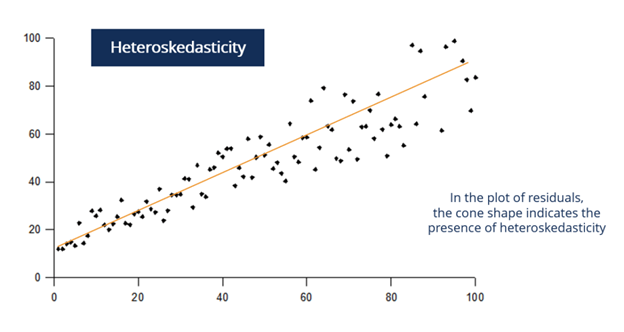
\includegraphics[width = .75\textwidth,keepaspectratio]{./figs/heteroskedasticity.png}
% \end{frame}


\end{document}